\chapter{Determining the Effect of Personality Types on Human-Agent Interactions}
\label{ch4}

\section{Introduction}
Agents are used nowadays to help with people's everyday life in many ways. For example, an agent could help travelers find the cheapest ticket for a specific flight, or get elders their medications. Thus, it is not surprising that people have feelings about agents. It is reported that humans show empathy towards robots  \cite{lewis2013}, evidenced by measuring their emotional and neurological change when they watched videos of dinosaur robots being abused. However, people's feelings towards agents are not always positive. There's a long-existing controversy about how the agents would behave after they have too much intelligence. Some people are afraid that robots, which are a kind of agents, might kill humans if they are intelligent enough and their interests conflict with humans' interests, despite the rule of "A robot may not injure a human being or, through inaction, allow a human being to come to harm", as stated in "The Three Laws of Robotics" \cite{asimov2004robot}. Along with the technology development of many different kinds of agents, questions have risen: will humans behave preferentially towards other humans or agents? It is known that humans' personality types have impact on interactions between humans, but how about the human-agent interaction? Will a human's personality type have an impact on his/her decisions regarding other humans and agents? If we discover some relationship between personality types and decisions, how could we use these information to help with everyday life? In order to answer these questions, we must determine a human's personality type first.

\subsection{Personality Types}
There are different methods to test personality types. A famous psychometric questionnaire to reveal a person's personality type is the Myers-Briggs Type Indicator (MBTI) assessment \cite{myers1980gifts}. Myers used four dichotomies in MBTI theory, as shown in Table \ref{dich}. 

\begin{table}[!t]
\caption{MBTI Dichotomies}
\label{dich}
\centering
\begin{tabular}{|c|}
\hline
Extraversion (E) - Introversion (I)\\ \hline
Sensing (S) - iNtuition (N)\\ \hline
Thinking (T) - Feeling (F)\\ \hline
Judging (J) - Perception (P)\\ \hline
\end{tabular}
\end{table}

The result of the MBTI questionnaire is a four-letter personality type, with one letter coming from one of the four dichotomies. For example, a person with type INFP means he/she is introverted, intuitive, friendly, and more likely to probe the environment. 

We chose the Keirsey Temperament Sorter-II (KTS-II) \cite{keirsey1998please}, which is closely associated with MBTI. KTS-II classifies people into four temperament groups according to two basic dimensions of personality: what people say (communication) and what people do (action). There are two types of communication: concrete people talk about reality while abstract people talk about ideas, shown by the columns of Table \ref{kts}. Similarly, there are two types of action: cooperative and utilitarian. Cooperative people do what's right and utilitarian people do what works, as shown by the rows in Table \ref{kts}.    

\begin{table}[!t]
\caption{KTS-II dimentions}
\label{kts}
\centering
\begin{tabular}{|c|c|}
\hline
Abstract Cooperator (Idealist)& Concrete Cooperator (Guardian)\\ \hline
Abstract Utilitarian (Rational)& Concrete Utilitarian (Artisan)\\ \hline
\end{tabular}
\end{table}

The temperaments are Artisan, Guardian, Rational, Idealist, whose names come from Plato's book \emph{The Republic}. They each have different traits \cite{keirseywebsite}:
\begin{itemize}
\item[-]\textit{Idealists} speak mostly of what they hope for and imagine might be possible for people, and they want to act in good conscience, always trying to reach their goals without compromising their personal code of ethics. Examples of the Idealists are Mohandas Gandhi and Princess Diana. 
\item[-]\textit{Guardians} speak mostly of their duties and responsibilities, of what they can keep an eye on and take good care of, and they're careful to obey the laws, follow the rules, and respect the rights of others. Examples of the Guardians are George Washington and Mother Teresa.   
\item[-]\textit{Rationals} speak mostly of what new problems intrigue them and what new solutions they envision, and always pragmatic, they act as efficiently as possible to achieve their objectives, ignoring arbitrary rules and conventions if need be. Examples of the Rationals are Hillary Clinton and Stephen Hawking.
\item[-]\textit{Artisans} speak mostly about what they see right in front of them, about what they can get their hands on, and they will do whatever works, whatever gives them a quick, effective payoff, even if they have to bend the rules. Examples of the Artisans are Michael Jordan and Marilyn Monroe.
\end{itemize}

Each temperament has four variants, as shown in the first two columns in Table \ref{ktsmbti}. The third column in Table \ref{ktsmbti} shows the MBTI types corresponding to the KTS-II types. KTS-II describes behaviorial patterns while MBTI describes what people have in mind, which makes KTS-II suitable for our experiments in theory. For convenience, we sometimes use the letters from the MBTI dichotomies to denote the KTS-II personality types in this chapter.  

\begin{table}[!t]
\caption{KTS-II temperament vs MBTI type}
\label{ktsmbti}
\centering
\begin{tabular}{|c|c|c|}
\hline
\textbf{KTS-II temperament} & \textbf{KTS-II character type} & \textbf{MBTI type}\\ \hline
\multirow{4}{*}{Artisan (SP)} & Promoter&ESTP\\ \cline{2-3}
&Crafter&ISTP\\ \cline{2-3}
&Performer & ESFP\\ \cline{2-3}
&Composer & ISFP\\ \hline

\multirow{4}{*}{Guardian (SJ)} & Supervisor & ESTJ\\ \cline{2-3}
&Inspector&ISTJ\\ \cline{2-3}
&Provider & ESFJ\\ \cline{2-3}
&Protector & ISFJ\\ \hline

\multirow{4}{*}{Rational (NT)} & Fieldmarshal&ENTJ\\ \cline{2-3}
&Mastermind & INTJ\\ \cline{2-3}
&Inventor & ENTP\\ \cline{2-3}
&Architect & INTP\\ \hline

\multirow{4}{*}{Idealist (NF)} & Teacher & ENFJ\\ \cline{2-3}
&Counselor & INFJ\\ \cline{2-3}
&Champion & ENFP\\ \cline{2-3}
&Healer & INFP\\ \hline

\end{tabular}
\end{table}

\subsection{The Cake-Cutting Game}
After the human subjects get their personality types through the KTS-II test, they are asked to play the "Who Gets More Cake?" game, which is related to the classic cake-cutting game. 

In the classic cake-cutting game, players want to divide a cake in such a way that all of them believe they have received a fair amount of the cake. There are two basic measurements for a solution of the cake-cutting problem: fairness and envy-freeness. Fairness means anyone gets at least the amount that he believes is fair, while envy-freeness means anyone believes no one gets more than he has and he won't want to exchange his cake with others. If the cake is divided between two players, there is a fair and envy-free solution, which is to have one player cut the cake into two pieces and the other player choose his piece of the cake first. For three players, Selfridge-Conway discrete procedure \cite{robertson1998cake} can be used to provide a fair and envy-free solution. However, our focus here is whether humans of different personality types act differently towards an agent, not dividing the cake perfectly with fairness and envy-freeness. We add a "leftover cake giveaway" part to the cake-cutting game in our "Who Gets More Cake?" game, which will be described in detail in section \ref{ch4:exp}. 

The rest of the chapter is organized as follows. In section \ref{ch4:related}, we introduce some related work. In section \ref{ch4:exp} and \ref{ch4:results}, the experiments are described in detail and the results are analyzed. In section \ref{ch4:conclusion}, we draw the conclusion.

\section{Related Work}
\label{ch4:related}
Reeves and Nass \cite{Reeves1996} claimed that people were inclined to treat media, usually computers in their studies, as if they were real people or real places. Thus we have the hypothesis that the personality types of humans would influence their behavior towards other humans and agents, just like in the interactions between humans.

Bartneck, Hoek, Mubin, and Mahmud \cite{Bartneck2007} used "iCat" robots of different intelligent levels to test whether humans treat the robots differently. They showed that the robots' intelligence had a significant influence on the humans' decision in the measurement of their hesitation time to switch off the robot. While they investigated the influence of different intelligence levels towards humans' decision, we try to figure out whether the personality type of a human influences his decisions towards a person or an agent. 

Many researchers who investigated the influence of personality types towards humans' decisions. For example, Schmitt, Shupp, Swope, and Mayer \cite{Schmitt2008} used MBTI test to get personality types and let the human subjects play the ultimatum game. In the ultimatum game, there are two players: a proposer and a responder. The proposer first makes an offer on how to divide a given amount of money, then the responder could accept or reject. The money is divided according to the offer if the responder accepts, but none of them gets anything if the responder rejects. They discovered that the "Thinking (T)" types made lower offers than those characterized as "Feeling (F)" types and "Extraversion (E)" types indicated a willingness to accept offers that was less than "Introversion (I)" types. Peever, Johnson and Gardner \cite{Peever2012} used the Five Factor Model to test the personality types and discovered the games a person preferred was related to his personality type.

Personality traits including those in Five Factor Model \cite{digman1990} and some other traits, such as public self-consciousness and shyness are considered by Von der Putten, Kramer, and Gratch \cite{vonderputten2010}. In their study, subjects recruited through a website interacted with a virtual agent. They found that some personality traits, such as agreeableness, extraversion, approach avoidance, were related to humans' behavior, while some traits, gender, and age didn't affect the results.

We presented the questions of this chapter in the mixed human-agent society and some experimental results in \cite{du2013} \cite{du2013iat}. This chapter studies the impact of humans' personality types towards their behavior, while it is different from other studies because of three reasons: 
\begin{itemize}
\item[-]Other than MBTI or Five Factor Model, we used KTS-II test in our study, which broadens the domain of possible explanations of the influences that personality types could bring to human behavior.
\item[-]Many researchers considered the interaction between a person and an agent, sometimes just between humans, while we considered a human interacts with both a simulated human and an agent at the same time, showing the different aptitudes the human has towards the simulated human and the agent.
\item[-]We explored a different experimental setting from previous studies, which may bring new conclusions since conclusions based on previous studies might only be applied to certain studies. We developed a new game and try to figure out how humans would behave in this situation.
\end{itemize}
           


% An example of a floating figure using the graphicx package.
% Note that \label must occur AFTER (or within) \caption.
% For figures, \caption should occur after the \includegraphics.
% Note that IEEEtran v1.7 and later has special internal code that
% is designed to preserve the operation of \label within \caption
% even when the captionsoff option is in effect. However, because
% of issues like this, it may be the safest practice to put all your
% \label just after \caption rather than within \caption{}.
%
% Reminder: the "draftcls" or "draftclsnofoot", not "draft", class
% option should be used if it is desired that the figures are to be
% displayed while in draft mode.
%
%\begin{figure}[!t]
%\centering
%\includegraphics[width=2.5in]{myfigure}
% where an .eps filename suffix will be assumed under latex, 
% and a .pdf suffix will be assumed for pdflatex; or what has been declared
% via \DeclareGraphicsExtensions.
%\caption{Simulation Results}
%\label{fig_sim}
%\end{figure}

% Note that IEEE typically puts floats only at the top, even when this
% results in a large percentage of a column being occupied by floats.


% An example of a double column floating figure using two subfigures.
% (The subfig.sty package must be loaded for this to work.)
% The subfigure \label commands are set within each subfloat command, the
% \label for the overall figure must come after \caption.
% \hfil must be used as a separator to get equal spacing.
% The subfigure.sty package works much the same way, except \subfigure is
% used instead of \subfloat.
%
%\begin{figure*}[!t]
%\centerline{\subfloat[Case I]\includegraphics[width=2.5in]{subfigcase1}%
%\label{fig_first_case}}
%\hfil
%\subfloat[Case II]{\includegraphics[width=2.5in]{subfigcase2}%
%\label{fig_second_case}}}
%\caption{Simulation results}
%\label{fig_sim}
%\end{figure*}
%
% Note that often IEEE papers with subfigures do not employ subfigure
% captions (using the optional argument to \subfloat), but instead will
% reference/describe all of them (a), (b), etc., within the main caption.


% An example of a floating table. Note that, for IEEE style tables, the 
% \caption command should come BEFORE the table. Table text will default to
% \footnotesize as IEEE normally uses this smaller font for tables.
% The \label must come after \caption as always.
%
%\begin{table}[!t]
%% increase table row spacing, adjust to taste
%\renewcommand{\arraystretch}{1.3}
% if using array.sty, it might be a good idea to tweak the value of
% \extrarowheight as needed to properly center the text within the cells
%\caption{An Example of a Table}
%\label{table_example}
%\centering
%% Some packages, such as MDW tools, offer better commands for making tables
%% than the plain LaTeX2e tabular which is used here.
%\begin{tabular}{|c||c|}
%\hline
%One & Two\\
%\hline
%Three & Four\\
%\hline
%\end{tabular}
%\end{table}


% Note that IEEE does not put floats in the very first column - or typically
% anywhere on the first page for that matter. Also, in-text middle ("here")
% positioning is not used. Most IEEE journals/conferences use top floats
% exclusively. Note that, LaTeX2e, unlike IEEE journals/conferences, places
% footnotes above bottom floats. This can be corrected via the \fnbelowfloat
% command of the stfloats package.



\section{Experiment}
\label{ch4:exp}
As mentioned before, our experiment contains two phases: 
\begin{itemize}
\item[-]Test the subjects' personality types using KTS-II.
\item[-]The subjects play the "Who Gets More Cake?" game. 
\end{itemize}
Figure \ref{ch4:fmodelhai} shows the model of the human-agent interaction system. A subject shown on the left takes the personality test and plays the game with the other two players on a computer and the computer will send the result data to a database for further analysis. The upper right corner shows a simulated human who is faked by an agent. 

\begin{figure}
\centering
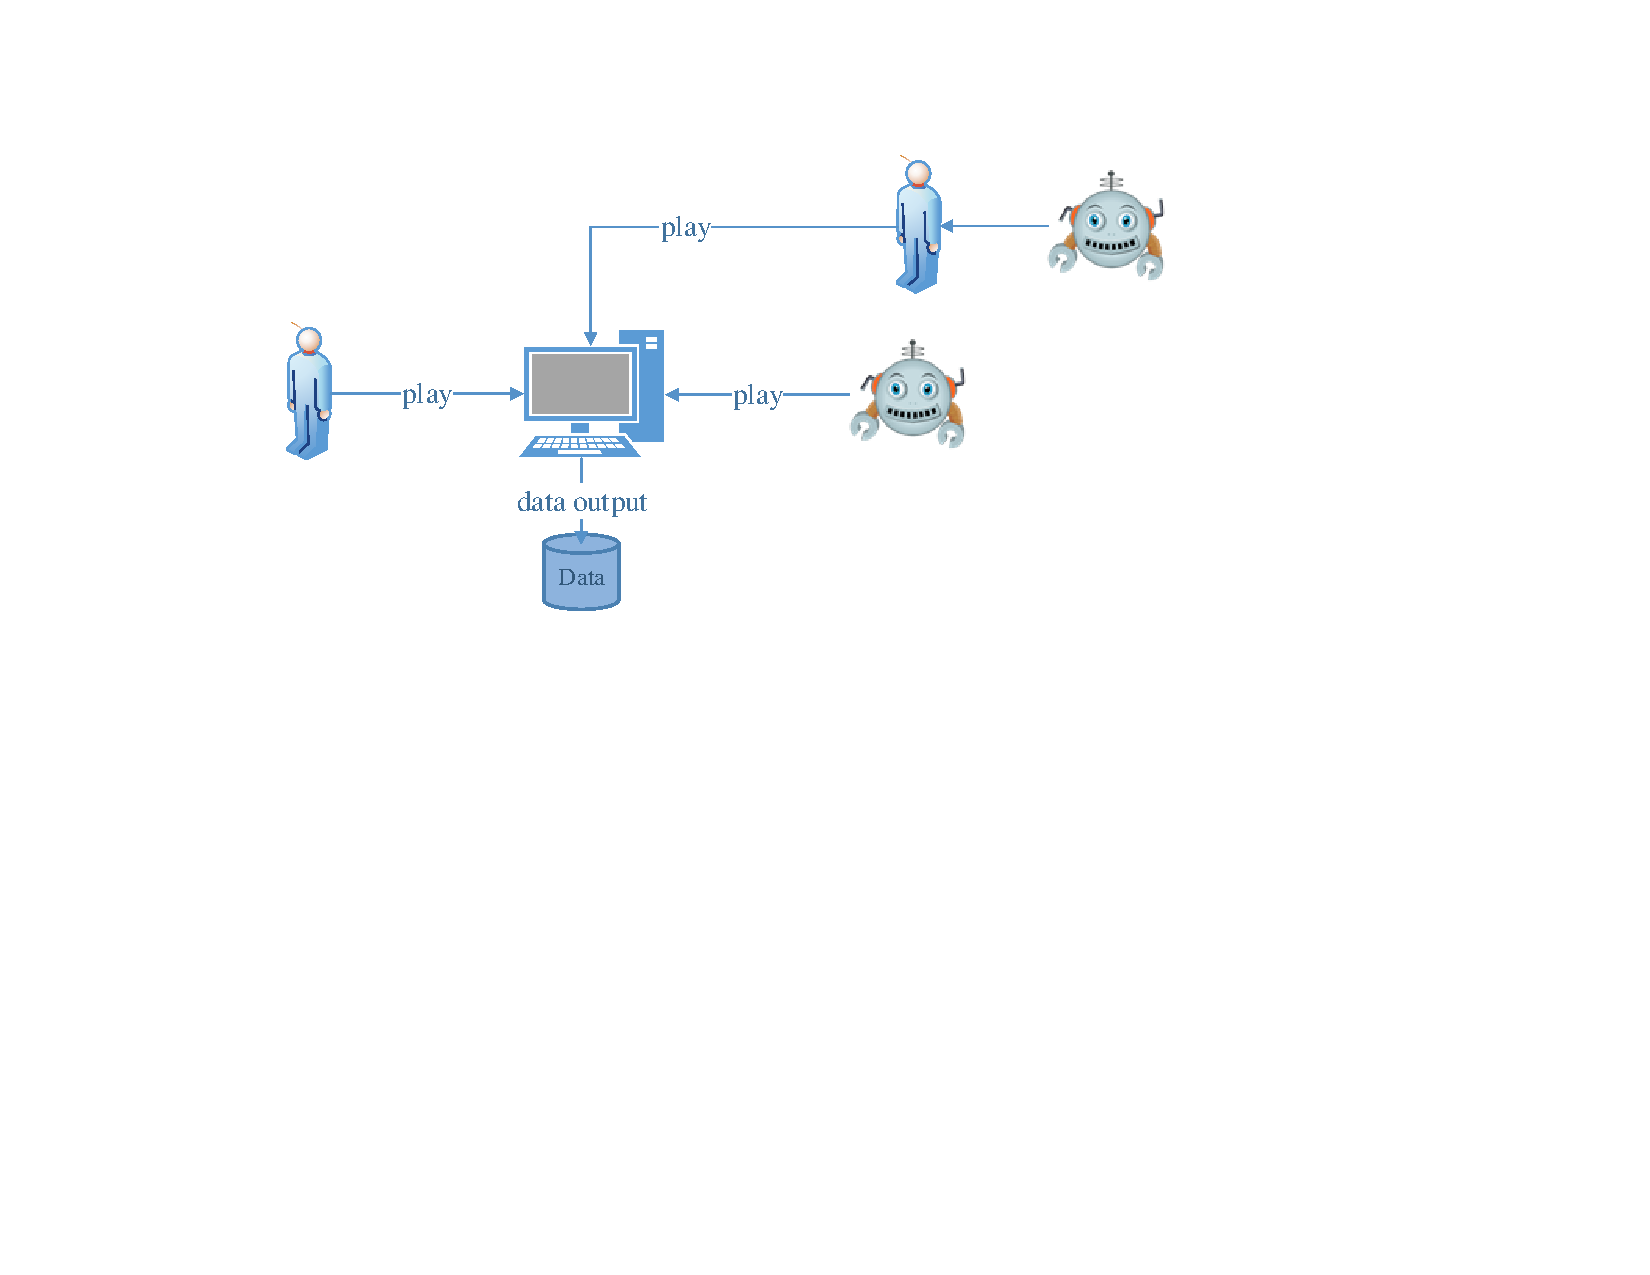
\includegraphics[scale=0.8]{chap4/chap4-model.pdf}
\caption{The model of the human-agent interaction system}
\label{ch4:fmodelhai}
\end{figure}

In our "Who Gets More Cake?" game, we have a cake for three players to divide. One player is the human subject/participant, one player is a simulated human, and the third player is an agent/robot (the robot has a way to convert the cake into the energy it needs to move). The participant was told he was playing with another person and a robot, but actually a simulated human and an agent for the reason of experimental control. Each player indicates how he would like to cut the cake into three pieces by drawing two lines/cuts on his own picture of the cake. Thus, we will have six lines on the cake in total after the players draw the lines. We then follow a protocol proposed by Iyer and Huhns \cite{Iyer2005}, which is proved to be fair for dividing a resource among n agents, to decide how the cake is divided: whoever has drawn the left-most cut will get the left side of the cake from the edge to this cut. Of the remaining two players, whoever has drawn the right-most cut will get the right side of the cake from this cut to the right edge. The third player will get the portion in the middle indicated by that player's two cuts. Note that all players will get one of the pieces that they indicated, as proved in  \cite{Iyer2005}. 

After the cake is divided, no player would want to trade with others, because they would get a piece that is smaller than the one they drew on the cake. However, there will be one or two portions of the cake left. To make the game more real, the participants were told one player would then be chosen randomly to give the remaining portions of the cake to one of the other players in each game. In fact, the participants were asked to whom they would give the leftover cake in every game. They could only give the leftover cake to either the simulated human or the agent, but not themselves. Each participant was asked to play the game three times, each time with a different cake and with a different simulated human. To play the part of a human as real as possible, our simulated human has different names in three games and their names are neutral to eliminate the bias of sex. At the beginning of each game, participants were asked to type a greeting sentence to the simulated human and the simulated human will type some greetings too. It takes our simulated human some time to think and draw cuts on the cake, each game with different amount of delay to mimic human thinking.

\section{Results}
\label{ch4:results}
73 non-computer science students with age around 20 who have little technological background participated in the experiment. They took the KTS-II personality test and played the game after being told the rules of the game. 58 of them played all three rounds of the game. In total, they played 197 games. We measure four criteria: 
\begin{itemize}
\item[-]The number of games in which the participants give the leftover cake to the simulated human, denoted by $N_{human}$;
\item[-]The number of games in which the participants give the leftover cake to the agent, denoted by $N_{agent}$;
\item[-]The number of participants who give the leftover cake to the same player (either the simulated human or the agent) in the three games they played, denoted by $N_{same}$;
\item[-]The number of participants who give the leftover cake to different players in the three games they played, denoted by $N_{diff}$.
\end{itemize}

The first two criteria measure the tendency that a participant would like to choose either a person or an agent under some circumstances, which might indicates whether he would like to interact with a person or an agent, and the last two criteria measure the consistency of his choice. For the last two criteria, we only consider the participants who finished all three games.
     
To deal with the personality type results, we first need to understand how to interpret KTS-II test. KTS-II provides a questionnaire based on seventy questions, each with two options indicating the two aspects of a certain dichotomy. There are ten questions for E (Extraversion)-I (Introversion) dichotomy and twenty questions each for the other three dichotomies. A personality type depends on how many options you selected for the two aspects of each dichotomy. If a person chooses the same number of options for the two aspects of any dichotomy, an "X" will appear for that dichotomy. For example, if a person choose 5 options for E (Extraversion) and 5 options for I (Introversion), his personality type will have an "X" in the E (Extraversion)-I (Introversion) dichotomy, such as XSTJ. If this happens, the person should read both ESTJ and ISTJ's descriptions and choose the one more like himself. In our experiments, a few participants have one or more "X"es in their personality types. We handle this by counting them as 1/2 person for one "X" situation for each possible type, 1/4 person for two "X"es situation for each possible type, and so on. For example, the above person with personality type XSTJ is counted as 1/2 person with type ESTJ and 1/2 person with type ISTJ.

In order to investigate how the personality types influence the choices the participants make, we introduce several statistic criteria to do evaluation: 
\begin{itemize}
\item[-]Pearson's chi-squared test ($\chi^{2}$ test) or Fisher's exact test, which evaluates the degree of independence between two nominal variables. 
\item[-]$Cram\acute{e}r's\:V\:(V)$, which is an effect size measure of association between two nominal variables.
\item[-]Goodman and Kruskal's lambda, which help us to understand whether knowing a person's personality would help to predict his choice in the game ($\lambda_{1}$) and vice versa ($\lambda_{2}$).
\end{itemize}  

\subsection{Tendency Results}
We calculated first two criteria for all the participants as a whole and have 
\begin{equation}
N_{human}=133,\:N_{agent}=64.
\end{equation} 

The data shows the participants give the leftover cake to the simulated human in most games, which is twice as many as those in which it is given to the agent. We grouped the data by sixteen MBTI types. The data is shown in Table \ref{ch4:tendencyOfMBTI}, which reveals that almost people of all the types give more leftover cakes to the humans than to the agents, which reveals their different aptitude towards the humans and the agents. Champion (ENFP), one of the Idealists, gives the leftover cakes to the simulated human 6 times than they give to the agent. On the other hand, Crafter (ISTP), one of the Artists, give more cake to the agent. $|\Delta|$ in the table is the absolute difference of $N_{human}$ and $N_{agent}$,
\begin{equation}
|\Delta|=|N_{human}-N_{agent}|.
\end{equation}
$d_r$ is the percentage difference, which is the relative difference in percentage calculated by the following formula:
\begin{equation}
d_r=\dfrac{|\Delta|}{(N_{human}+N_{agent})/2}
\end{equation}
The data is heterogeneous and it's hard to discover the pattern among all the sixteen personality types. That's one clue of suggesting us to group them in some way and analyze the results.

\begin{table}[!t]
% increase table row spacing, adjust to taste
%\renewcommand{\arraystretch}{1.3}
\caption{Tendency Results of MBTI Types}
\label{ch4:tendencyOfMBTI}
\centering
\begin{tabular}{|c|c|c|c|c|}
\hline
\textbf{MBTI type} & \boldmath{$N_{human}$} &\boldmath{$N_{agent}$} & \boldmath{$|\Delta|$} & \boldmath{$d_{r}$} \\ \hline
ESTJ	&8.25	&6.75	&1.5	&5\%	\\ \hline
ISTJ	&17.25	&9	&8.25	&16\%	\\ \hline
ESFJ	&12.875	&3.5	&9.375	&29\%	\\ \hline
ISFJ	&16.875	&7.25	&9.625	&20\%	\\ \hline
ESTP	&7	&4.5	&2.5	&11\%	\\ \hline
ISTP	&2	&2.75	&0.75	&8\%	\\ \hline
ESFP	&8.625	&3.5	&5.125	&21\%	\\ \hline
ISFP	&6.125	&2.75	&3.375	&19\%	\\ \hline
ENFJ	&3.375	&2.5	&0.875	&7\%	\\ \hline
INFJ	&5.875	&2	&3.875	&25\%	\\ \hline
ENFP	&12.625	&2	&10.625	&36\%	\\ \hline
INFP	&8.125	&5	&3.125	&12\%	\\ \hline
ENTJ	&7	&2.25	&4.75	&26\%	\\ \hline
INTJ	&8	&2.25	&5.75	&28\%	\\ \hline
ENTP	&2.25	&2	&0.25	&3\%	\\ \hline
INTP	&6.75	&6	&0.75	&3\%	\\ \hline
\end{tabular}
\end{table}


\subsubsection{KTS-II Temperaments Tendency Results}
Thus, we calculated the same criteria for the four KTS-II temperaments, as shown in Table \ref{kts1ct} and criteria for each two aspects of the four dichotomies, as shown in Table \ref{dimen1}. 

Now we want to see whether the KTS-II temperaments have significant influence on the choices the participants made. Our data fits the conditions of Pearson's $\chi^{2}$ test.  Following the test procedure, we stated the null hypothesis as follows: 

$H_{0}$: The participants' KTS-II temperaments and the choices they made are independent.

Then we represent the data in a contingency table as in Table \ref{kts1ct}, where $R_{total}$ describes row total and $C_{total}$ describes column total. The participants choices, as we observed, are called observed frequencies ($O_{freq}$) in statistics.

\begin{table}[!t]
% increase table row spacing, adjust to taste
%\renewcommand{\arraystretch}{1.3}
\caption{Observed Frequencies of Four Temperaments}
\label{kts1ct}
\centering
\begin{tabular}{|c|c|c|c|c|c|}
\hline
\boldmath{$O_{freq}$} &\textbf{Guardian} & \textbf{Artisan} &\textbf{Idealist} & \textbf{Rational} & \boldmath{$R_{total}$} \\ \hline
\boldmath{$N_{human}$} &55.25 &23.75 &30 &24 &133\\ \hline
\boldmath{$N_{agent}$} &26.5 &13.5 &11.5 &12.5 & 64\\ \hline
\boldmath{$C_{total}$} &81.75 &37.25 & 41.5 &36.5 &197\\ \hline
\end{tabular}
\end{table}

Our hypothesis is that there is no relationship between the participants' temperaments and their choices, which means they give the leftover cake to the simulated human or the agent randomly (i.e., with equal probability). Based on this hypothesis, we obtain the expected frequencies ($E_{freq}$) according to the following formula, which are the frequencies if we don't consider the factor of personality. For example, let's consider the expected frequency of $N_{human}$ for Guardian. If we don't know a person's personality, then he should give the leftover cake to the simulated human by the probability of $133/197$. With a total number of 81.75 people, the number of people who give the leftover cake to the simulated human should be $81.75*133/197=55.19$. The expected frequencies are shown in Table \ref{kts1ct2}.
\begin{equation}
E_{freq}=C_{total}*R_{total}/T
\end{equation}
For a specific cell in the expected frequency table, $C_{total}$ in the above formula is the column total for the column of that cell, while $R_{total}$ is the row total for the column of that cell. $T$ in the formula is the number of games played in total, which is 197 in our case. 

\begin{table}[!t]
% increase table row spacing, adjust to taste
%\renewcommand{\arraystretch}{1.3}
\caption{Expected Frequencies of Four Temperaments}
\label{kts1ct2}
\centering
\begin{tabular}{|c|c|c|c|c|}
\hline
\boldmath{$E_{freq}$} &\textbf{Guardian} & \textbf{Artisan} &\textbf{Idealist} & \textbf{Rational} \\ \hline
\boldmath{$N_{human}$} &55.19 &25.15 &28.02 &24.64 \\ \hline
\boldmath{$N_{agent}$} &26.56 &12.10 &13.48 &11.86 \\ \hline
\end{tabular}
\end{table}

We use the following formula to calculate $\chi^{2}$:
\begin{equation}
\chi^{2}=\sum_{0<i<m,\:0<j<n}
\frac{(O_{freq}(i,j)-E_{freq}(i,j))^{2}}{E_{freq}(i,j)},
\end{equation}
where $O_{freq}(i,j)$ and $E_{freq}(i,j)$ denote the observed frequencies and expected frequencies in the table cell of $i$th row and $j$th column. $m$ and $n$ represents the total row number and total column number. The statistical results are  
\begin{equation}
\chi^{2}=0.72,\:P=0.87,\:V=0.06.
\end{equation}
$P$ is one-tailed (right-tail) probability value for a chi-square test (i.e., the area under the chi-square distribution from the chi-square value to positive infinity), given the chi-square value and the degree of freedom, which can be calculated through a lookup table or an online tool. The degree of freedom $df$ is the number of values in the table that are free to vary given existing constrains. In our table, $R_{total}$ and $C_{total}$ are the constrains fixed for each row and column. In the table, we only need to vary the contents of 3 cells and the contents of the rest cells could be decided then. Thus, the degree of freedom is 3 in our case. $V$ is calculated using the following formula:
\begin{equation}
\sqrt{\frac{\chi^{2}}{T*(k-1)}},
\end{equation}
where $T=197$ and $k=2$, which is the smaller number of the number of rows and the number of columns in the table. 

The meaning of the result is that we are $1-P$ (in the form of percentage) sure to reject the null hypothesis. Normally significant level of 0.05 or 0.1 is used, which means if $P<0.05$ or $P<0.1$ we can reject the hypothesis. In our case, $P>0.05$ and there is 13\% probability that we could reject the hypothesis, which is very low. Thus we can't reject the null hypothesis, which means we can't say there is a relationship between the participants' temperaments and their choices. $V$ is an effect size measure which shows the inter-correlation of the variables. In this case, it measures the relationship between the participants' KTS-II temperaments with their choices. According to the convention, $V<0.1$ means negligible relationship. In our case, $V=0.06$ means the association between the KTS-II temperaments and the choices is negligible.   

Percentage deviation, which measures the degree to which observed frequencies differs from the expected frequencies, is calculated as follows:
\begin{equation}
PD(i,j)=\frac{O_{freq}(i,j)-E_{freq}(i,j)}{E_{freq}(i,j)}.
\end{equation}

Table \ref{kts1pd} shows the percentage deviation of the KTS-II temperaments' tendency results, from which we could see that people with different temperaments behave very differently. Artisans and Idealists are deviated more from the general public than the other two temperaments. The Guardians act just like an average person. By an average person, we refer to an imaginary person who will act as our reference data shows. For example, if this person plays our game for 197 times, he would probably end up with giving the leftover cake 133 times to the simulated human and 64 times to the agent.

\begin{table}[!t]
% increase table row spacing, adjust to taste
%\renewcommand{\arraystretch}{1.3}
\caption{Percentage Deviation of Four Temperaments}
\label{kts1pd}
\centering
\begin{tabular}{|c|c|c|c|c|}
\hline
\textbf{Percentage Deviation} &\textbf{Guardian} & \textbf{Artisan} &\textbf{Idealist} & \textbf{Rational} \\ \hline
\boldmath{$N_{human}$} &0.1\% &-5.6\% &7.1\% &-2.6\% \\ \hline
\boldmath{$N_{agent}$} &-0.2\% &11.6\% &-14.7\% &5.4\% \\ \hline
\end{tabular}
\end{table}

At last we use Goodman and Kruskal's lambda to measure the proportional reduction in error. For example, in our case, the estimated probability of correct prediction when predicting a person's choice without knowing his temperament is 
\begin{equation}
p_{1}=\frac{133}{197}=0.68,
\end{equation}
while estimated probability of correct prediction when predicting what choice a person will make knowing his temperament is
\begin{equation}
p_{2}=\frac{55.25+23.75+30+24}{197}=0.68.
\end{equation}
Goodman and Kruskal's lambda of predicting choice on the basis of temperament is 
\begin{equation}
\lambda_{1}=\frac{(1-p_{1})-(1-p_{2})}{1-p_{1}}=0,
\end{equation} 
which means there is no difference whether or not knowing a person's temperament when predicting his choice. Also we found out lambda of predicting a person's temperament from his choice ($\lambda_{2}$), which is calculated according to a similar way as that of $\lambda_{1}$, is 0, meaning knowing a person's choice won't do any good to predicting the his temperament.       

To give a hint of how the participants' choices of each dichotomy varies, table \ref{dimen1} shows the tendency results of four dichotomies, where $PD_{human}$ is the percentage deviation of $N_{human}$ and $PD_{agent}$ is the percentage deviation of $N_{agent}$. We could see that the biggest difference from what is supposed to be with our equal probability assumption happens in the T-F dichotomy.

\begin{table}[!t]
% increase table row spacing, adjust to taste
%\renewcommand{\arraystretch}{1.3}
\caption{Tendency Results and Percentage Deviation of Four Dichotomies}
\label{dimen1}
\centering
\begin{tabular}{|c|c|c|c|c|}
\hline

\textbf{MBTI dichotomy} & \boldmath{$N_{human}$} &\boldmath{$N_{agent}$} & \boldmath{$PD_{human}$} & \boldmath{$PD_{agent}$} \\ \hline
E (Extraversion)&	62&	27 &3.2\% &-6.6\%\\ \hline
I (Introversion)&	71&	37 &-2.6\% &5.5\%\\ \hline
S (Sensing)&	79&	40 &-1.7\% &3.5\% \\ \hline
N (iNtuition)&	54&	24 &2.5\% &-5.3\% \\ \hline
T (Thinking)&	58.5&	35.5 &-7.8\% &16.2\% \\ \hline
F (Feeling)&	74.5&	28.5 &7.1\% & -14.8\%\\ \hline
J (Judging)&	79.5&	35.5 &2.4\% & -5.0\%\\ \hline
P (Perception)&	53.5&	28.5 &-3.4\% & 7.0\% \\ \hline
\end{tabular}
\end{table}

Then we investigated how MBTI dichotomies influence the choices the participants made. Following the same procedure, first we stated the null hypothesis for each dichotomy as follows:
\begin{itemize}
\item[-]For E-I dichotomy: The participants' types in E-I dichotomy and their choices are independent;
\item[-]For S-N dichotomy: The participants' types in S-N dichotomy and their choices are independent;
\item[-]For T-F dichotomy: The participants' types in T-F dichotomy and their choices are independent;
\item[-]For J-P dichotomy: The participants' types in J-P dichotomy and their choices are independent.
\end{itemize} 

Table \ref{dimen1results} shows the statistic results for each dichotomy. From the table we could see that in T-F dichotomy, there is 87\% possibility, which is close to the standard of rejecting the null hypothesis with a significance level of 0.1, to reject the null hypothesis. Still, we can't reject the null hypothesis, but we probably could see it get rejected with more experiments and draw a conclusion that the personality in T-F dimension has something to do with the participants' choices based on statistics. For other dimensions, there is no evidence to lead to the conclusion that we should reject the null hypothesis and say there is a relationship between a certain dichotomy and the choices. 

Also, we could see from $Cram\acute{e}r's\:V$ there's a weak relationship between T-F dichotomy and the choices, and negligible relationship between any other dichotomy and the choices in the whole population based on our samples. $\lambda_{2}$ for T-F dichotomy is 0.07, which means that we could reduce 7\% error when predicting a person's temperament with his choice known compared to that with his choice not known.     

\begin{table}[!t]
% increase table row spacing, adjust to taste
%\renewcommand{\arraystretch}{1.3}
\caption{Statistical Results of Four Dichotomies for Tendency}
\label{dimen1results}
\centering
\begin{tabular}{|c|c|c|c|c|c|}
\hline
\textbf{MBTI Dichotomy} &\boldmath{$\chi^{2}$} & \boldmath{$P$} &\boldmath{$V$} & \boldmath{$\lambda_{1}$} & \boldmath{$\lambda_{2}$} \\ \hline
E-I &0.34 &0.56 &0.04 &0 &0\\ \hline
S-N &0.17 &0.68 &0.03 & 0 &0 \\ \hline
T-F &2.28 &0.13 &0.11 & 0 & 0.07\\ \hline
J-P &0.33 &0.57 &0.04 &0 &0 \\ \hline
\end{tabular}
\end{table}


\subsection{Consistency Results}
Next, we measure the consistency of the participants' choices. First we calculated the consistency criteria:
\begin{equation}
N_{same}=18,\:N_{diff}=40.
\end{equation} 
We could see that more than two thirds of participants give the leftover cake to different players in three games, which means they don't always prefer the simulated human or the agent. Similar to the tendency results, we grouped the $N_{diff}$ and $N_{same}$ data according to temperaments and dichotomies, shown in the first three columns in Table \ref{kts2} and Table \ref{dimen2}. We could consider the consistency as "fairness" in the sense that the participants try to behave "fairly" by giving the leftover cake to the simulated human and the agent in three repetitions of the game, rather than to only one of them.    

It is not suggested to use Pearson's $\chi^{2}$ test if there are small expected frequency values, so we use Fisher's exact test here to perform analysis similar to Pearson's $\chi^{2}$ test for data in Table \ref{kts2} and it turns out $P$ is very close to 1. We also perform Pearson's $\chi^{2}$ test to get an approximate $V$ value. Our null hypothesis is as follows: 

$H_{0}$: The participants' KTS-II temperaments and the consistency results of their choices are independent.

The statistical results are as follows:
\begin{equation}
\chi^{2}=0.22,\:V=0.06,\:\lambda_{1}=0,\:\lambda_{2}=0.
\end{equation}
It shows that there is no significant dependence between the participants' KTS-II temperaments and the consistency of their choices. A person's temperament has little association with the consistency of his choices. Knowing a person's temperament or the consistency of his choices won't do any help to the prediction of the consistency of his choices or his temperament.

\begin{table}[!t]
% increase table row spacing, adjust to taste
%\renewcommand{\arraystretch}{1.3}
\caption{Consistency Results and Percentage Deviation of Four Temperaments}
\label{kts2}
\centering
\begin{tabular}{|c|c|c|c|c|}
\hline
\textbf{KTS-II Temperament}& \boldmath{$N_{same}$} & \boldmath{$N_{diff}$} & \boldmath{$PD_{same}$} & \boldmath{$PD_{diff}$}\\ \hline
Guardian& 7.75&	16.5 & 3.0\% & -1.3\%\\ \hline
Artisan& 3.25&	7.5 & -2.6\% & 1.2\% \\ \hline
Idealist& 3&	8.5 &-15.9\% &7.2\%\\ \hline
Rational& 4&	7.5 &12.1\% &-5.4\% \\ \hline
\end{tabular}
\end{table}

Then we investigated how MBTI dichotomies influence the consistency of the choices that the participants made. Following the same procedure, first we stated the null hypothesis for each dichotomy as follows:
\begin{itemize}
\item[-]For E-I dichotomy: The participants' types in E-I dichotomy and the consistency of their choices are independent;
\item[-]For S-N dichotomy: The participants' types in S-N dichotomy and the consistency of their choices are independent;
\item[-]For T-F dichotomy: The participants' types in T-F dichotomy and the consistency of their choices are independent;
\item[-]For J-P dichotomy: The participants' types in J-P dichotomy and the consistency of their choices are independent.
\end{itemize} 

\begin{table}[!t]
% increase table row spacing, adjust to taste
%\renewcommand{\arraystretch}{1.3}
\caption{Consistency Results and Percentage Deviation of Four Dichotomies}
\label{dimen2}
\centering
\begin{tabular}{|c|c|c|c|c|}
\hline
\textbf{MBTI dichotomy} & \boldmath{$N_{same}$} & \boldmath{$N_{diff}$} & \boldmath{$PD_{same}$} & \boldmath{$PD_{diff}$}\\ \hline
E (Extraversion)&	9&	15.5 &18.4\% &-8.3\%\\ \hline
I (Introversion)&	9&	24.5 &-13.4\% &6.0\%\\ \hline
S (Sensing)&	11&	24 & 1.3\% & -0.6\%\\ \hline
N (iNtuition)&	7&	16 & -1.9\% &0.9\%\\ \hline
T (Thinking)&	8.5&	20 &-3.9\% &1.8\%\\ \hline
F (Feeling)&	9.5&	20 & 3.8\% &-1.7\%\\ \hline
J (Judging)&	11.5&	22 &10.6\% &-4.8\%\\ \hline
P (Perception)&	6.5 &18 &-14.5\% &6.5\%\\ \hline
\end{tabular}
\end{table}

\begin{table}[!t]
% increase table row spacing, adjust to taste
%\renewcommand{\arraystretch}{1.3}
\caption{Statistical Results of Four Dichotomies for Consistency}
\label{dimen2results}
\centering
\begin{tabular}{|c|c|c|c|c|c|}
\hline
\textbf{MBTI Dichotomy} &\boldmath{$\chi^{2}$} & \boldmath{$P$} &\boldmath{$V$} & \boldmath{$\lambda_{1}$} & \boldmath{$\lambda_{2}$} \\ \hline
E-I & 0.64 & 0.42 & 0.11 & 0 & 0\\ \hline
S-N & 0.01 & 0.92 & 0.01 & 0 & 0\\ \hline
T-F &0.04 & 0.84 & 0.03 & 0 & 0\\ \hline
J-P & 0.4 & 0.53 & 0.08 & 0 & 0\\ \hline
\end{tabular}
\end{table}

Table \ref{dimen2}, where $PD_{same}$ and $PD_{diff}$ denote the percentage deviation of $N_{same}$ and $N_{diff}$, gives us a hint of how the observed data deviates from what should be with equal possibility assumption. E-I and J-P dichotomies deviates more than the other two dichotomies. The statistical results are shown in Table \ref{dimen2results}, based on which we couldn't reject any of the null hypothesis and say any dichotomy and the consistency results are not independent. Besides, knowing a person's dichotomies or the consistency of his choices won't do any help to the prediction of the consistency of his choices or dichotomies. However, $Cram\acute{e}r's\:V$ shows there is a weak association between E-I dichotomy and the consistency of the choices. In conclusion, being fair is more important than personality.  
 

\section{Conclusion}
\label{ch4:conclusion}
In this chapter, we try to investigate whether humans' behavior towards other humans and agents is related to their personality types. We have seventy-three students participated in the experiments, by taking the KTS-II test and then playing the "Who Gets More Cake?" game. 

We discovered that humans of different personality types behave differently towards other humans and agents. For example, Artisans and Idealists act more deviated from an average person; it's very likely that T-F dichotomy is not independent with the tendency results. This provides a clue in many agent-related applications. For example, an Idealist has to partner
with an agent/robot as his personal assistant due to business
reasons. As an Idealist, he is inclined to interact with humans more and agents less, thus he might choose an robot with less talking
or interactions needed. In the next stage, we may discover agents of which personality type could cooperate well with a certain kind of person, which could be used in many domains, such as elder's personal care, team formation and so on. 

Currently our experiments shows little clue of making predictions based on a person's personality. In the future, we expect that more students participate in an updated version of this experiment to draw more reliable conclusion based on our statistical criteria and explore other possibilities. Also, the personality types of the simulated human and the agent are not considered yet. We expect to find a way to integrate this factor into the future experiments.  
